\documentclass[12pt]{article}
\usepackage{geometry}
\geometry{paperwidth=5.31in, paperheight=3in, bottom=10mm}

\usepackage{tzplot}
\usepackage{chemfig}
\pagenumbering{gobble}
\def\hash{\textbf{\#}}
\usepackage{amsmath}
\usepackage{electrons}
\usepackage{mathtools}
\def\dt{\tikz\tzdot*(0, 0)(5pt);}
%\chemsetup{modules=all}

\begin{document}

\begin{center}
\textbf{Hybridization}
\end{center}

\begin{enumerate}

\item[\hash] $\chemfig{CH_4}$\\ \underline{\textcolor{black!95}{According to VBT}}

\begin{align*}
& C \quad\quad && H\\
& [He]2s^2 2p^2  \quad\quad && 1s^1 \\
& \subshells{{2s:2}}~\subshells{{2p:11}{:0}} \quad \xrightarrow{\text{excitation}} \quad && \subshells{{2$s^1$:1}} ~ \subshells{{2$p^3$:111}}\\
\end{align*}

\pagebreak

\item[\dt] $\chemfig{CH_4}$ has 4 $\sigma$-bond
\item[\dt] $2s-1s$ Overlap $\Rightarrow ~$ $1~\sigma$-bond 

\item[\dt] $2p-1s$ Overlap $\Rightarrow ~$ $3~\sigma$-bonds at angle of $90^\circ$

\item[\dt] Strength: $2s-1s < 2p-1s$ 

%\pagebreak

\item[\hash] \textbf{Hybridization:-} Intermixing of pure atomic orbitals and form new hybrid orbitals \\
Eg. - $\chemfig{CH_4}$


\pagebreak
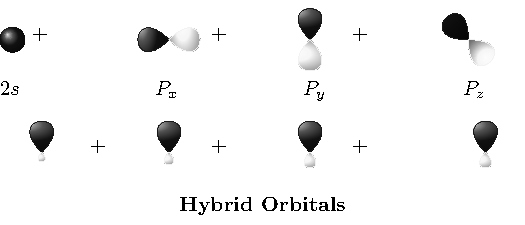
\includegraphics[scale=1]{./orbitals/main.pdf}

\item[\dt] Hybridization = $\sigma + \text{lone pair}$

\item[\dt] \textbf{Example:-}	$sp^3 = s + p_x + p_y + p_z$ 
\pagebreak

\item[\dt] $sp < sp^2 < sp^3$

\item[\dt] \textbf{Example:-} \chemfig{PCl_5}
\begin{center}
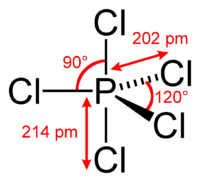
\includegraphics[scale=15]{pcl5.png}
\end{center}

\pagebreak
\item[\dt] \textbf{Example:-} \chemfig{PF_5}
\begin{center}
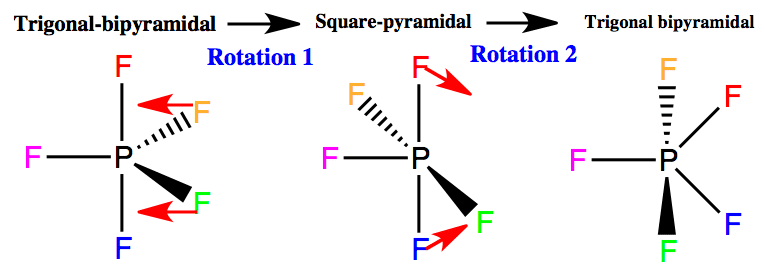
\includegraphics[scale=0.3]{pf5.png}
\end{center}

\pagebreak
$~$\hfill

\pagebreak

$~$\hfill

\pagebreak

$~$\hfill

\pagebreak

$~$\hfill
\pagebreak

$~$\hfill
\pagebreak



\end{enumerate}





\end{document}